\documentclass{elbioimp2}
\usepackage[utf8]{inputenc}

\usepackage[backend=biber,style=vancouver]{biblatex}
\usepackage{csquotes}
\usepackage[braket]{qcircuit}
\usepackage{float}

\title{The state of Quantum Computing in 2025}
% \shorttitle{Short version of title}
\author{Adam Prior.\affiliation{UrbanFox, Dublin, Ireland}} 
\shortauthor{A. Prior.}
% \elbioimpreceived{19 Sept 2025}  
% \elbioimppublished{19 Sept 2025}
% \elbioimpfirstpage{1}
% \elbioimpvolume{x}
% \elbioimpyear{20xx}
 
\addbibresource{bibliography.bib}

\begin{document}
\setcounter{secnumdepth}{2}


\maketitle

\begin{abstract}
  This paper provides an accessible overview of the current state of quantum computing technologies
  as of September 2025. Aimed at readers with a technical background but no prior experience in quantum
  computing, it reviews foundational concepts, historical advancements, and leading hardware and software platforms. The paper
  also discusses practical challenges, potential applications, and the outlook for future developments in the field.

  \keywords{Quantum Computing; Qubits; Decoherence; robotics}
\end{abstract}

\section{. Introduction}
Define Quantum Advantage here.
Define Some other terms here.

todo: add to historical section that Shor's algorithm is somewhat of a benchmark for quantum computing


\section{. Historical Advancements in Quantum Computing}
The first mentions of quantum computation can be traced as far back as the early as 1980s.
In 1980, mathematician Yuri Manin discussed the concept of a quantum computer in his paper
`Computable and Uncomputable'\cite{Manin1980}. Richard Feynman, in 1982, published a paper
`Simulating physics with computers' introducing the idea of simulating
quantum systems using quantum computers\cite{Feynman1982}, highlighting the limitations
of classical computers at simulating the exponentially growing state space of quantum
systems and how quantum systems can be more efficiently simulated. 

Given these initial few years of defining work, the field began
to gain traction, followed by another \textit{10 years} of foundational theoretical developments.
In 1985, David Deutsch further developed the quantum computing theory by rigorously defining the
Universal Quantum Turing Machine (the quantum analog of a classical Turing machine) capable of
performing any computation that a classical computer can, but more efficiently for certain problems\cite{Deutsch1985}. 
Further theoretical advancements continued with contributions from, reversible quantum computation by Paul Benioff between
1985-1987\cite{BBenioff1987}, the first proposal of a physically realizable quantum computer 
using atoms and photons in 1998\cite{Yamamoto1998}, and attempts to define quantum complexity 
classes in 1989\cite{Bernstein1993} which would eventually lead to the definition of 
Bounded-Error Quantum Polynomial Time (BQP) problems, an important class of problems in complexity
theory that can be efficiently solved by quantum computers in polynomial time.

It was not until 1992 that the first quantum algorithm was proposed by Deutsch and Jozsa\cite{Deutsch1992},
demonstrating that quantum computers could solve certain problems more efficiently than classical computers 
(quantum advantage). While this algorithm has very limited practical applications, it paved the way for more 
impactful algorithms.
The most famous of these is Shor's algorithm, proposed by Peter Shor in 1994\cite{Shor1994}. Shor's algorithm 
is an efficient quantum algorithm for integer factorization in polynomial time, versus the best-known classical
algorithms which run in sub-exponential time. This algoirithm in some sense `proved' the potential of quantum computing
to solve practical problems that are intractable for classical computers, particularly in the context of cryptography, as
many encryption schemes rely on the difficulty of factoring large integers. 
Another significant algorithm is Grover's algorithm, proposed by Lov Grover two years later\cite{Grover1996}, providing
quadratic speedup for unstructured search problems.

While these algorithms demonstrate the theoretical potential of quantum computers, they would be useless without
the ability to assemble a physical quantum computer. Around the same time as these algorithmic developments,
experimental researchers were developing the first real qubits and quantum gates. The first experimental demonstration
of a quantum logic gate was realised in 1995 by a team using an electromagnetic trap to confine ions in place to form a two-qubit
system. The energy levels of the ions are used to represent the qubit states (|0⟩ and |1⟩), while laser pulses are used 
to manipulate these states. The team successfully implemented a controlled-NOT (CNOT) gate, which is a fundamental quantum gate
universal quantum gate used in many quantum algorithms\cite{Monroe1995}. 
One might define this point in time as the take-off point in the history of quantum computing as it was demonstrated, roughly in parallel,
to be both theoretically computationally advantageous (for certain classes of problems) and experimentally realisable and a large acceleration
in research and development followed. Over the next decade experiments would demonstrate  more complex gates, and increased amount of qubits 
(8 qubit registers by December 2005)\cite{https://www.nature.com/articles/nature04279}, and even new quantum systems that can implement qubits 
such as superconducting states, nuclear spins, quantum dots and even photon polarization\cite{Monroe1995}. Theoretical advancements also continued, with the 
development of quantum error correction codes and various proofs of principle for quantum algorithms that further highlighted feasability and
limitations.

Up to this point, it is well known that quantum computers suffer from an extreme scaling problems. Qubits are extremely sensitive to their environment
and suffer badly from quantum decoherence which limits the rate at which additional qubits can be added to a system before the entire system becomes unstable
highlighting why it took so long to scale beyond only a few qubits. Table~\ref{tab:qubit_counts} summarizes some of the key leaps in qubiit counts over the years.

\begin{table*}[b]
\centering
\begin{tabular}{|c|c|l|}
\hline
\textbf{Year} & \textbf{Qubit Count} & \textbf{Description} \\
\hline
1995 & 2 & First experimental demonstration of a quantum logic gate using trapped ions\cite{Monroe1995} \\
\hline
2001 & 7 & Implementation of Shor's algorithm on a 7-qubit NMR quantum computer\cite{Vandersypen2001} \\
\hline
2005 & 8 & Demonstration of an 8-qubit register using trapped ions\cite{https://www.nature.com/articles/nature04279} \\
\hline
2011 & 5 & D-Wave Systems announced a 512-qubit quantum annealer\cite{DWave2011} \\
\hline
2016 & 16 & IBM unveiled a 16-qubit superconducting quantum processor\cite{IBM2016} \\
\hline
2017 & 20 & Google announced a 20-qubit superconducting quantum processor\cite{Google2017} \\
\hline
2019 & 53 & Google's Sycamore processor achieved quantum supremacy with 53 qubits\cite{Arute2019} \\
\hline
2020 & 65 & Honeywell announced a 65-qubit trapped-ion quantum computer\cite{Honeywell2020} \\
\hline
2021 & 127 & IBM unveiled a 127-qubit superconducting quantum processor\cite{IBM2021} \\
\hline
2022 & 433 & IonQ announced a 433-qubit trapped-ion quantum computer\cite{IonQ2022} \\
\hline
2023 & 1000+ & Various companies announced plans for quantum processors with over 1000 qubits\cite{Various2023} \\
\hline
2024 & 2000+ & Continued advancements with processors exceeding 2000 qubits\cite{Various2024} \\
\hline
2025 & 5000+ & Leading companies project quantum processors with over 5000 qubits\cite{Various2025} \\
\hline
\end{tabular}
\caption{Key advancements in qubit counts from 1995 to 2025 and their corresponding platforms.}\label{tab:qubit_counts}
\end{table*}


% "The next major advancement in quantum computing came in 2009 with the proposal of topological qubits
% by Alexei Kitaev\cite{Kitaev2003}. Topological qubits are designed to be more robust against local sources of decoherence by encoding information in global properties of the system
% rather than local states. This approach promised to significantly reduce error rates and improve the scalability of quantum computers. While still in the experimental stage, topological qubits represent a promising avenue for building more practical and scalable quantum computers."


\section{. Fundamentals of Quantum Computing}
In order to properly understand the current state of quantum computing, it is important to first understand
some of the fundamental concepts. What exactly is a qubit? What is superposition and entanglement? What is a quantum gate?

\subsection{. Qubits and their construction}
For the average reader without a background in quantum mechanics, but with at least some technical background in computing,
a qubit can be thought of as the quantum analog of a classical bit. When we use the term `classical', we specifically mean 
non-quantum, as in the type of computing that underpins all modern computers today. A classical bit represents the fundamental 
unit of information in classical computing and is binary in nature, meaning that a bit exists in either one of two states, usually
represented as 0 or 1. In classical physics, it is straightforward to encode a bit's state as either 0 or 1. Usually this is done
using voltage levels, where a high voltage might represent a 1 and a low voltage a 0. An important point to state at this point
is that a classical bit can only exist in one of these two states at any given time. In classical physics there is no such thing as being both high and low voltage at the same time. It is either one or the other.

Similarly a qubit is also a binary unit of information, but it operates according to the principles of quantum mechanics. There are many quantum mechanical systems that can be used to physically realise a qubit, and generally, any two-level quantum system can technically be used as a qubit. Consider, for example, the spin angular momentum of an electron. This `spin' can take strictly two values: `up' or `down', which can be used to represent the 0 and 1 states of a qubit. Other physical systems that can be used to realise qubits include the polarization states of photons, energy levels of atoms or ions, and superconducting circuits. We are not limited to just electronic spins but a rich variety of physical systems can be used to implement qubits, each with its own advantages and challenges. Such systems include but are not limited to:
\begin{itemize}
  \item Trapped Ions electronic states
  \item Superconducting states (charge, flux, or phase)
  \item Photonic Qubits (polarization states, number of photons, etc)
  \item Quantum Dots (electron localization states, spin)
  \item Nuclear Spins (nuclear magnetic resonance spin)
\end{itemize}

When we consider that the underlying quantum system is being used as just a different way to encode a binary state, it might be tempting to think of a qubit as just a more complex representation of a classical bit. However, the actual power of of quibits lies in their ability to exist in a state called a \textit{quantum superposition}, which is a fundamental principle of quantum mechanics.


\subsection{. Quantum States, Superposition and Entanglement}
In the realm of quantum mechanics we represent the state of a quantum system using a special notation called Bra-ket notation. In this notation, the up state is represented as |0⟩ and the down state as |1⟩. As mentioned previously, however, unlike a classical bit, a qubit can exist in a combination (superposition) of both states simultaneously. For those who are mathematically inclined, this means that a qubit can be in a state that is a linear combination of |0⟩ and |1⟩, represented mathematically as:
\begin{equation}
  |\psi\rangle = \alpha|0\rangle + \beta|1\rangle
\end{equation}

where $\psi$ just means `the state of the qubit'. The coefficients $\alpha$ and $\beta$ are complex numbers that represent the probability amplitudes of the qubit being in the |0⟩ and |1⟩ states, respectively. This expression for the superposition, given that the complex coefficients are continuous values, show us that the qubit has an uncountably infinite amount of states it can be in. 
\begin{figure}[htbp]
  \centering
  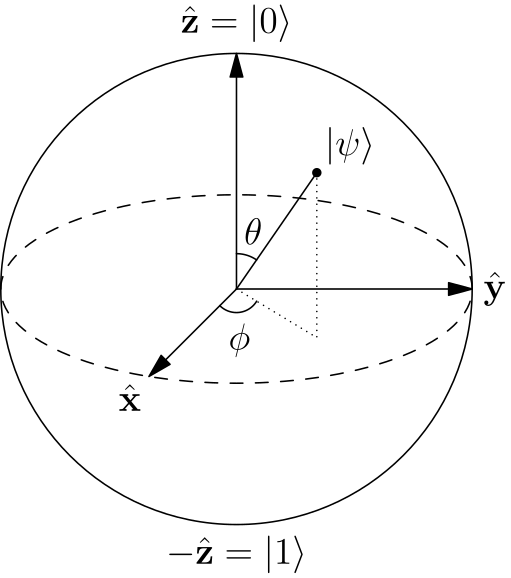
\includegraphics[width=0.75\columnwidth]{assets/bloch-sphere.png}
  \caption{The Bloch Sphere representation of a qubit. Any point on the surface of the sphere represents a valid qubit state, with |0⟩ and |1⟩ at the poles. The angles $\theta$ and $\phi$ determine the specific superposition state.}
  \label{fig:bloch-sphere}
\end{figure}
The probabilities of measuring the qubit to be in either state are given by the squares of the magnitudes of these coefficients. In some sense they represent the `weight' of each state in the superposition, the likelihood that measuring the qubit will give that particular state, as in quantum mechanics, the act of measurement causes the qubit to `collapse' into one of the base states (either |0⟩ or |1⟩) with probabilities determined by these coefficients. It is this superposition that enables quantum computers to perform certain computations more efficiently than classical computers as these complex coefficients can interfere constructively or destructively during quantum computations, allowing quantum algorithms to amplify the probabilities of correct answers while suppressing incorrect ones.

The nature of superposition also leads to the concept of \textit{entanglement}, another fundamental property of quantum mechanics. When two qubits become entangled, the state of one qubit becomes directly correlated to the state of the other, regardless of the distance between them. This means that measuring one qubit instantly determines the state of the other qubit. Entanglement is a key resource in many quantum algorithms and protocols, enabling phenomena such as quantum teleportation and superdense coding. It is also a crucial component in achieving quantum advantage, as it allows for correlations that are not possible in classical systems as there is no classical analog to entanglement, it is a purely quantum mechanical phenomenon.

As the coefficients $\alpha$ and $\beta$ are complex numbers, they have both a magnitue and a phase, and it is this phase that allows for interference effects to occur due to relative phase differences between qubit states. Maintining stable relative phases is critical for the proper functioning of quantum algorithms, and is measured by a property called coherence time, which is the time over which a qubit can maintain its quantum state before loss of information to the environment (decoherence) occurs. The global coherence of a multi-qubit system is particularly important, as quantum algorithms often rely on the interference of amplitudes across multiple qubits to achieve their computational advantage. Two important metrics used to quantify the coherence of qubits are $\tau_1$ and $\tau_2$ times. $\tau_1$, or relaxation time, measures how long a qubit can stay in an excited state before it decays to its ground state due to energy loss to the environment. $\tau_2$, or dephasing time, measures how long a qubit can maintain its phase coherence before interactions with the environment cause it to lose its quantum information. Both $\tau_1$ and $\tau_2$ times are critical for the performance of quantum computers, as they determine how long quantum information can be reliably stored and manipulated.

\subsection{. Quantum Gates}

It's all well and good to be able to create qubits and understand their properties, in order to perform computations we need a way to manipulate these qubits and perform quantum gate operations on them. Quantum gates are the quantum analogs of classical logic gates. While classical logic gates could be interpreted as performing operations that flip or combine bits in their restrictied classical space, quantum gates are represented mathematically by matrices operating on the state (vectors) of the qubits, performing flips, rotations, entanglements and other transformations in the much larger quantum state space. This makes more sense when considering the geometric representation of a qubit on the Bloch sphere (see Figure.~\ref{fig:bloch-sphere}), where quantum gates can be visualized as rotations of the qubit state vector on this sphere.

\begin{figure}[h]
  \centering
  \scalebox{1}{
    \Qcircuit{
      \lstick{\ket{q_1}} & \gate{H} & \ctrl{1} & \gate{S} & \qw \\
      \lstick{\ket{q_2}} & \ctrl{2} & \ctrl{0} & \ctrl{1} & \qw \\
      \lstick{\ket{q_3}} & \qw & \qw & \gate{Y} & \qw \\
      \lstick{\ket{q_4}} & \targ & \gate{X} & \qw & \qw \\
    }
  }
  \caption{Example of a simple 4-qubit quantum circuit. Each horizontal line represents a qubit, and the symbols show basic operations that can be performed on them such as the Hadamard gate (H), controlled-NOT gate (CNOT), phase gate (S), Pauli-X gate (X), and Pauli-Y gate (Y).}
\end{figure}

In practice, the experimental implementation of quantum gates depends on the physical system used to realise the qubits. For example, in superconducting qubits, microwave pulses are used to manipulate the energy levels of the qubits, while in trapped ion systems, laser pulses are used to control the internal states of the ions. Common single-qubit gates include the Pauli-X, Y, and Z gates (which correspond to bit-flip and phase-flip operations), as well as the Hadamard gate (which creates superposition). Multi-qubit gates, such as the CNOT (Controlled-NOT) gate, are essential for creating entanglement between qubits and enabling more complex quantum operations. Given that gate operations are actual physical operations, they take a finite duration of time. The time taken to perform a gate operation, known as the gate time $\tau_g$, is important in the context of quantum algorithms, as it must be much shorter than the coherence times ($\tau_1$ and $\tau_2$)(see practical challenges section).

\subsection{. Decoherence, Errors, and Correction}
In an actual quantum computer, we are far from the ideal mathematical situation of qubits being perfectly coherent, noise free, and decoupled from the environment. In practice, the quantum states required are incredibly delicate, generally requiring the system to be supercooled to near absolute zero temperatures, and isolated from all external influences. Even still, it is impossible to remove all sources of noise, and as such, the system is subject to decoherence. Decoherence is the proceess by which a quantum system loses its quantum properties due to interactions with its environment. This can occur through various mechanisms, such as thermal fluctuations, electromagnetic interference, or imperfections in the qubit fabrication process. Decoherence leads to the loss of superposition and entanglement, effectively collapsing the qubit states into classical states and destroying the quantum information they carry. This is not a limitation of hardware alone, but a fundamental property of quantum mechanics itself. As stated earlier, the coherence times $\tau_1$ and $\tau_2$ are critical metrics that quantify how long a qubit can maintain its quantum state before decoherence occurs. As we add more qubits to the system, the global coherence of the multi-qubit becomes exponentially more fragile and susceptible to decoherence, making it increasingly challenging to maintain the quantum information across the entire system. Decoherence ultimately results in the occurrence of errors during quantum computations as the global state collapses unpredictably.

Decoherence is not the only source of error in quantum computations. The quantum gate operations themselves are also subject to imperfect operations and thus have some probability of failure. For example, attempting to perform an X gate on a qubit in the |0⟩ state might not always successfully flip it to the |1⟩ state due to imperfections in the control pulses or interactions with the environment during the gate operation. This is known as gate error. Gate fidelity is a measure of how accurately a quantum gate performs the intended operation, and it is typically quantified using metrics such as the average gate fidelity. As a rule of thumb, gate fidelities above 99\% are generally considered good, but for practical quantum computing, even higher fidelities (e.g., 99.9\% or better) are often required\cite{99.9percent-required-fidelity}.

To mitigate the effects of decoherence and gate errors, quantum error correction techniques are employed. Error correction involves encoding the quantum information across multiple physical qubits to create logical qubits that are more robust against errors. This is typically done using quantum error-correcting codes, such as the surface code or the Steane code, which can detect and correct certain types of errors without directly measuring the quantum information itself (which would collapse the state). Implementing error correction requires additional qubits and gate operations, which adds complexity to the quantum computer. The overhead for error correction can be significant, often requiring an order of magnitude more physical qubits to create a single logical qubit. However, this is essential for achieving fault-tolerant quantum computing, where computations can be performed reliably even in the presence of noise and errors.


\section{. Practical Challenges in Quantum Computing}
\subsection{1. Decoherence and Noise}
As stated in the previous section, the fragility of quantum states plays a huge role in the accuracy of quantum computations. Qubits interact unavoidably with their environments, leading to decoherence that destroys superpositions and entanglement, which are essential for quantum advantage and reducing the error rates of quantum gates. Minimizing decoherence and noise is one of the biggest challenges in building practical quantum computers. The scaling effect of decoherence and noise is particularly problematic as the number of qubits increases, making it exponentially more difficult to maintain coherence across the entire system as we enter the realm of hundreds to thousands of qubits.


\subsection{. Gate Fidelity and Speed}
Given the coherence windows $\tau_1$ and $\tau_2$, these set a hard limit on how many gate operations can be performed before the quantum information is lost. As a real example in trapped ion systems, which can have exceptionally long coherence times of the order of seconds or longer, single-qubit gate times can be on the order of microseconds, while two-qubit gates can take tens to hundreds of microseconds. For a 50 second coherence time and 500$\mu s$ gate time, this allows for only 100,000 gate operations before decoherence occurs and destroys the computation. When considering a practical algorithm like Shors algorithm for integer factorization, this number seems far more than enough when considering the trvial example of factoring the number 15 (4-bits) into its factors of 3 and 5. But entering the regime of RSA encryption where we are dealing with 2048-bit numbers to be factorized, we are looking at the order of anywhere from billions to trillions of gate operations. Thus, faster gate operations are desirable to maximize the number of operations that can be performed within the coherence time. However, increasing gate speed often comes at the cost of reduced gate fidelity, as faster gates can be more susceptible to control errors and noise. Thus, there a balance must be struck between gate speed and fidelity that must be carefully managed to optimize the performance of quantum computers.

Gate fidelity itself, an inverse measure of error rate of a gate operation, is a critical factor as even tiny errors in gate operations can accumulate over the course of a quantum computation, leading to incorrect results. Achieving high gate fidelities (e.g., above 99.9\%)\cite{99.9percent-required-fidelity} is essential for practical quantum computing, but this remains a significant challenge due to various sources of noise and imperfections in the control systems used to manipulate qubits. However we are already approaching and surpassing this threshold with fidelities exceeding 99.9\% in some platforms such as trapped ions, and germanium quantum dots\cite{Srinivas_2021,gemanium999}, and major advancements in 2025 in superconducting qubits have also pushed single gate fidelities reliably beyond 99.997\%\cite{PRXQuantum.5.040342}.

\subsection{. Error Correction, Fault Tolerance and the Logical-Physical Qubit Gap}

Given the probabilistic guarantee of gate faults and decoherence faults, as absolute requirement of quantum computing is to design the computations to be fault tolerant.
Acheiving fault tolerance in quantum computers opens its own entire area of research known as error correction with its own domain of difficulties.
The goal of error correction is to accept that faults are guaranteed to occur, and aims to detect them, and in turn correct them.
In general, this is achieved through the concept of a \textit{logical qubit}.

While actual physical qubits are capable of computation,
the probability of error is too high to achieve correct results for realistic problems. A logical qubit is an an {collection} of qubits that are used
for redundancy in the case of errors. We might then say, that one \textit{useful} quibit consists of multiple physical qubits. It is this logical qubit that quantum
computation is done with. The logical qubit becomes a fault tolerant qubit via the implementation of error correction codes which use the ensemle to correct errors that
occur in the logical qubit.

Many different error correction schemes exist, but leading schemes like surface codes or color codes require many physical qubits per logical qubit, leading to a huge overhead in the number of qubits required for practical quantum computing. In 2023, researchers at google showed experimentally that error rates could be reduced by using increased physical qubit counts\cite{GoogleQAI2023}. Specifically they showed that increasing the physical qubit count from 17 to 49 per logical qubit, the error rate decreased from 3.0\% to 2.9\% While this important result shows the potential for improving error rates through increased qubit counts, it also highlights the scale at which we might need to reach to achieve robust error correction. Modern error correction scheme estimates suggested that practical computing would hundreds to thousands of physical qubits per logical qubit, requiring a total number of physical qubits in the order of millions for a practical computation. This is often referred to as the logical-to-physical qubit gap, and it represents one of the biggest challenges in scaling up quantum computers to the sizes needed for practical applications. However, only in the last couple of years, huge strides have been made in developing super efficient error correction codes. 2024 research by  IBM reported the implementation of a new error correction code called the Gr$\o$ss code, which protected 12 logical qubits using only 288 physical qubits (24 qubits per logical qubit) for approximately one-million error correction cycles, demonstrating a significant reduction in the logical-to-physical qubit ratio\cite{FTQM2024} compared to other leading codes like surface code. Surface code, according to the IBM analysis, would require almost 3000 physical qubits to achieve the same task. 

Microsoft and Quintinium, also in 2024, announced similar low ratio logical qubits using only 30 physical to encode 4 logical qubits (7.5 physical per logical qubit) using their own error correction techniques. However their quantum system is limited to only 32 physical qubits, so while the ratio is impressive, the absolute number of logical qubits is still very small\cite{paetznick2024demonstrationlogicalqubitsrepeated}. However this highlights the rapid pace of advancements in error correction codes and the potential for more efficient schemes to significantly reduce the overhead required for fault-tolerant quantum computing.

While these results are promising, it is important to note that these are still early days in the development of practical error correction codes, and much work remains to be done to fully understand their performance and scalability in real-world quantum computing systems.

\subsection{. Time \& Space resource requirements for practical algorithms}
The particularly well known Shor’s algorithm is regularly used as the benchmark for quantum computing, as it is one of the most famous algorithms that demonstrates a clear quantum advantage over classical algorithms. It has been suggested in simpler implementations that Shor's algorithm for factoring an $n$-bit integer can be achieved with as `few' as $2n+3$ \textit{logical} qubits, with the number of gate operations required to achieve the factorization scaling as $O(n^3)$\cite{beauregard2003circuitshorsalgorithmusing}. Given RSA encryption 2048-bit integers this suggests RSA encryption breaking could be done with 4099 logical qubits, but in the order of tens-of-billions of gate operations (high gate depth) consisting of modular quantum additions, multiplications and fourier transforms generally performed sequentially. Given the current state of gate speeds and coherence times, this is far beyond the capabilities of current quantum computers as the system would decohere long before the computation could complete.

Further research has investigated trading space for time, and vice versa, i.e using circuits that require more qubits to reduce the overall gate depth, or circuits that use fewer qubits but require more gate operations. However, even with these optimizations, the resource requirements for practical implementations of Shor's algorithm remain extremely high. More recent estimates suggest that factoring a 2048-bit integer using Shor's algorithm would require on the order of 20 million physical qubits when considering error correction overheads and realistic gate fidelities in a computation taking around 8 hours\cite{Gidney_2021}. However no quantum computer with this physical qubit count is anywhere close to being built. On the flip side, trading time for space to minimize qubit counts, a 2024 paper proposed a method to factor a 2048-bit integer using only $n/2$ logical qubits (~1730) logical qubits, but at the cost of an extremely high gate depth requiring on the order of tens of trillions of operations\cite{10.1007/978-3-032-01878-6_13}. Even with optimistic gate speeds of 1 microsecond per gate and perfect error correction, this computation would take around 230 days to complete.

Considering the largest quantum computers to date, attention is generally brought to D-Wave's advantage system which boasts 5000+ qubits\cite{NatureQC2023}. However this does not actually operate as a universal quantum computer, specifically designed for optimization problems using quantum annealing. Despite this limitation, it highlights the vast discrepancy between current qubit counts and the requirements of millions for practical applications like breaking RSA encryption.


\subsection{. Qubit Connectivity, Control, and Engineering Challenges}

As quantum computers scale up, several engineering challenges emerge that impact their and scalability.

The physical layout of qubits is dictated by the underlying technology. Whether it's superconducting circuits, trapped ions, neutral atoms, or spin qubits each impose specific geometrical constraints on how qubits can interact. Most current platforms support only nearest neighbor connectivity, limiting the ability to perform entangling operations between distant qubits. While research into long range entanglement and modular interconnects is ongoing, practical quantum networks remain immature. As qubit density increases, cross talk becomes a significant issue, where imperfect isolation, physical proximity, and electromagnetic interference, amogst other effects can couple interactions across the system, degrading overall fidelity and thus increasing the likelihood of errors occuring.

Each qubit in a quantum processor requires precise calibration of its operating parameters, including laser frequencies, pulse shapes, and error mitigation settings. This complexity grows rapidly with the number of qubits, leading to a “complexity explosion” in control systems. The control systems required such as laser sources, and cryogenic infrastructure scale poorly in terms of energy consumption and system complexity. Additionally, hardware drift and environmental fluctuations necessitate frequent recalibration, reducing system uptime and computational efficiency.

The physical requirements for operating quantum hardware are extreme. Superconducting qubits, for example, require dilution refrigerators operating at temperatures near 10 mK, which are difficult to scale to support millions of control lines. Trapped ion and neutral atom systems depend on stable laser and vacuum setups, which are challenging to miniaturize and integrate. Fabrication of quantum devices also presents major hurdles: achieving uniform, and reproducible high fidelity qubits is an open challenge, with device variability causing significant error rates.

Together, these challenges necessitatethe need for advances not only in quantum theory and algorithms, but also in engineering, materials science, and systems integration to realize large-scale, fault-tolerant quantum computers.

\section{. Leading Quantum Hardware Platforms}

\section{. Future Outlook and Developments}
This document is a template for LATEX. Please use
the electronic version of this document as a template
when you produce your manuscript for submission to the
Nordic Machine Intelligence. The paper size is A4 (21 ×
29.7 cm).
The introduction section of your paper should include
the necessary background information, including an ade-
quate review of earlier findings and the justification for
conducting this study.
3.1. Qubits and their construction
All figures should be numbered consecutively with the
figure legend indented 0.5 cm on each side. See figure
commented fig for an example. Figures may be in color
or black and white and must be of such quality that they
produce clear and sharp printouts on an ordinary (color).
This document is a template for LATEX. Please use
the electronic version of this document as a template
when you produce your manuscript for submission to the
Nordic Machine Intelligence. The paper size is A4 (21 ×
29.7 cm).
The introduction section of your paper should include
the necessary background information, including an ade-
quate review of earlier findings and the justification for
conducting this study.
3.1. Qubits and their construction
All figures should be numbered consecutively with the
figure legend indented 0.5 cm on each side. See figure
commented fig for an example. Figures may be in color
or black and white and must be of such quality that they
produce clear and sharp printouts on an ordinary (color)

\newpage
\nocite{*}
\printbibliography
\end{document}
